\documentclass[12pt,a4paper,onecolumn,oneside,titlepage]{article}
\usepackage[utf8]{inputenc}
\usepackage[german]{babel}

\usepackage[T1]{fontenc}
\usepackage{amsmath}
\usepackage{amsfonts}
\usepackage{amssymb}
\usepackage{tikz}

\usepackage{footnote}
\makesavenoteenv{tabular}
\usepackage{wrapfig}
%for pseudocode
\usepackage{algorithm}
\usepackage{algpseudocode}
\usepackage{caption}
\usepackage{subcaption}
\usepackage{url}
\usepackage{booktabs}


\DeclareCaptionFormat{algor}{%
  \hrulefill\par\offinterlineskip\vskip1pt%
    \textbf{#1#2}#3\offinterlineskip\hrulefill}
\DeclareCaptionStyle{algori}{singlelinecheck=off,format=algor,labelsep=space}
\captionsetup[algorithm]{style=algori}

%return on a new line
\let\oldReturn\Return
\renewcommand{\Return}{\State\oldReturn}

\newcommand{\vars}{\texttt}
\newcommand{\func}{\textsc}
\newcommand\cursive[1]{\ensuremath{\mathcal{#1}}}


\newcommand\todo[1]{\textcolor{red}{#1}}
%\renewcommand\todo[1]{}


\author{Paul Walger}
\title{Heuristiken für das Entfernen von verbotenen Teilgraphen}
\makeindex
\begin{document}

\maketitle
\tableofcontents
\newpage
\begin{abstract}
Graphen so zu modifizieren, dass sie gewisse induzierte Teilgraphen nicht mehr enthalten, ist bis auf gewisse triviale Fälle NP-Vollständig.
 In dieser Arbeit erarbeiten wir schnelle Annäherungen und testen diese auf ihre Güte.
  
\end{abstract}
  
\section{Einleitung}

Graphen sind eine bildliche Darstellung von Beziehungen zwischen Objekten. Damit können sie eine Vielzahl von Problemen und Szenarien modellieren. Zum Beispiel können die Knoten Städte und die Kanten Zugverbindungen zwischen diesen Städten sein und somit wird der Graph das Zugnetzwerk von diesen Städten modellieren \cite{Nastos06}. 

\subsection{Motivation}
\label{sec:mot}
Wird nun ein System von Objekten mittels einem Graphen modelliert, hat der Graph ebenso wie das modellierte System gewisse Eigenschaften.

Eine solche Eigenschaft wäre, dass wenn ein Knoten $u$ mit einem anderen Knoten $v$ verbunden ist, so ist $u$ auch mit allen Nachbarn von $v$ verbunden. Graphen mit dieser Eigenschaft werden Cluster-Graphen  genannt. Diese bestehen aus einer oder mehreren Komponenten, in welcher jeder Knoten mit jedem Knoten verbunden ist.
Diese Cluster-Graphen lassen sich aber auch dadurch charakterisieren, dass sie gewisse Strukturen nicht besitzen und zwar, dass sie nicht den Graphen $P_3$ als einen induzierten Graphen haben. Der $P_3$ Graph ist in der Abbildung \ref{fig:mot-p3} zu sehen.
Einen $P_3$ als induzierten Teilgraphen zu haben, bedeutet, dass man jedem Knoten aus dem $P_3$ einen Knoten aus dem Graphen zuordnen kann, sodass gilt, wenn zwei Knoten im $P_3$ durch eine Kante verbunden sind, so sind auch die entsprechenden Knoten in dem Graphen durch eine Kante verbunden und umgekehrt.
 
Erklären lässt sich das an der Abbildung \ref{fig:mot}.
In dem Graphen $G_1$ in der Abbildung \ref{fig:mot-1} sehen wir, dass der Teilgraph mit den Knoten B,D und C ein von $P_3$ induzierter Subgraph ist, weil wir den Knoten $a$ dem Konten $B$, den Knoten $b$ dem Knoten $c$ und den Knoten $c$ dem Konten $D$ zuordnen können und die vorhin geforderte Eigenschaft gilt.
So sehen wir, dass im Graphen $P_3$ $a$ und $c$ verbunden ist und im  
$G_1$ auch $B$ und $D$ verbunden ist. Auch ist $B$ und $C$ in Graphen $G_1$ nicht verbunden und $a$ und $b$ ebenso.  Man kann überprüfen, dass die Voraussetzung für jede beliebiges Paar von Knoten geben ist und so ist der rot markierte Teilgraph ein von $P_3$ induzierte Teilgraph. 

Der Graph $G_2$ in der Abbildung \ref{fig:mot-2} hat keinen $P_3$ als induzierten Teilgraphen, weil wir nicht die Knoten vom $P_3$ zu Knoten in diesem Graphen zuordnen können und dabei unsere Voraussetzung erfüllt bleibt. Wenn wir also zum Beispiel, die Zuordnung vom Knoten $a$ zum Knoten $A$, $b$ zu $B$ und $c$ zu $C$ nehmen, sehen wir das Problem, dass wir eine Kante zwischen $A$ und $C$ haben aber keine Kante zwischen $a$ und $b$. Somit ist das keine gültige Zuordnung. Man kann aber auch nachvollziehen, dass egal wie die Zuordnung gewählt wird, es nicht möglich ist, die Bedingung zu erfüllen.

\begin{figure}
  \centering
 
  \begin{tabular}[c]{ccc}
    \begin{subfigure}[b]{0.32\textwidth}
      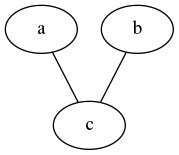
\includegraphics[scale=0.6]{dot/dot_mot_p3.png}
   
      \caption{Ein $P_3$ Graph }
      \label{fig:mot-p3}
   \end{subfigure}&
	 \begin{subfigure}[b]{0.32\textwidth}
	 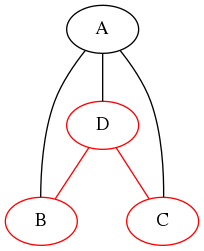
\includegraphics[scale=0.5]{dot/dot_mot_1.png}
	 
	    \caption{Graph $G_1$ mit einem von $P_3$ induzierten Teilgraphen.}
	    \label{fig:mot-1}
	  \end{subfigure}&
    \begin{subfigure}[b]{0.32\textwidth}
       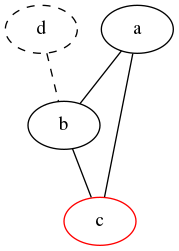
\includegraphics[scale=0.5]{dot/dot_explored_3.png}
	    \caption{Graph $G_2$ ohne einen induzierten $P_3$}
	    \label{fig:mot-2}
    \end{subfigure}
  \end{tabular}
  \caption{Cluster-Graphen}\label{fig:mot}
\end{figure}

Deshalb ist der Graph $G_2$ ein Cluster-Graph und hat eben diese besondere Eigenschaft, die auf zwei Weisen beschreiben werden kann: 1. Der Graph hat eine oder mehrere Komponenten wo jeder Knoten mit jedem Knoten verbunden ist und 2. Der Graph hat kein $P_3$ als einen induzierten Teilgraphen. Die erste Charakterisierung ist eine mehr natürliche und wir könnten zu einer solchen Beschreibung aus praktischen Beobachtungen über unsere Daten kommen, während die zweite eine eher mathematische ist und nicht immer intuitiv, aber dennoch sehr nützlich ist, weil wir eine Eigenschaft sehr leicht formulieren können.

In dieser Arbeit werden wir uns die Methoden anschauen, welche einen Graphen so modifizieren, so dass er eine bestimmte Eigenschaft hat. Viele Eigenschaften lassen sich, wie in dem vorherigen Beispiel mittels einer Charakterisation durch verbotenen Teilgraphen beschreiben.


\subsection{Definitionen}
\subsubsection{Notationen und Definitionen}
\label{sec:notation}
Mit Graphen sei im Folgenden stets ein ungerichteter, einfacher Graph gemeint. Wenn nicht anders angegeben ist, ist $G=(V,E)$ ein Graph, $V$ die Menge seiner Knoten und $E$ die Menge seiner Kanten.

Die Menge der Knoten des Graphen $G$ ist $V(G)$ und die Menge der Kanten des Graphen $G$ heißt $E(G)$. Die Nachbarschaft vom Knoten $u$ heißt $N(u)$, während $N^{*}(u)$ die Nachbarschaft von $u$ mit $u$ inklusive ist.

Sei $G = (V,E)$ ein Graph und $S \subseteq V$ eine beliebige Knotenmenge von $V$. 
Dann ist $G[S] = (S, E \cap \{\{u,v\} \,|\, u \in S \land w \in S\})$ der durch $S$ induzierte Subgraph von $G$.

Seien $H = (V_H,E_H)$ und $G =(V,E)$ zwei Graphen. Ein Subgraph-Isomorphismus von H nach G ist eine Funktion $f : V_H \rightarrow V$, sodass wenn $(u,v) \in E_H $ gilt, dann gilt auch $(f(u),f(v)) \in E$. $f$ ist ein induzierter Subgraph-Isomorphismus, wenn es auch gilt, dass wenn $(u,v) \notin E_H$, dann auch $(f(u),f(v)) \notin E$.

Seinen $G$ und $F$ Graphen, dann ist der Graph $G$ \textit{F}-frei, wenn es nicht \textit{F} als induzierten Subgraphen enthält.
Für eine Menge \cursive{F} von Graphen, heißt der Graph $G$ \cursive{F}-frei, wenn $G$ \textit{F}-frei ist für jeden \textit{F} $\in \cursive{F}$.

Die Editierdistanz $\Delta(G, \cursive{F})$ ist die minimale Anzahl von Kantenänderungen an G, damit G \cursive{F}-frei ist.\\ Die normierte Editierdistanz $\Delta^{*}(G, \cursive{F})$ ist $\frac{\Delta(G, \cursive{F})}{|E(G)|^{2}}$

Ein ungerichteter Graph $G$ heißt Wald, wenn er keinen Zyklus enthält. Ist der Graph $G$ zudem zusammenhängend, dann heißt er auch Baum. Jede Zusammenhangkomponente eines Waldes ist daher ein Baum.

TODO: Siehe \cite{Cai96} für eine Definition von FPT und Kernel.
\subsubsection{Problemstellung}
\label{sec:problem}
Das Problem, für das in dieser Arbeit Heuristiken entwickelt werden, kann wie folgt definiert werden:
\begin{quote}
  \textsc{\cursive{F}-Free Edge Editing}\newline
  \textbf{Eingabe:} Graph $G$, natürliche Zahl $k$, Menge von Graphen \cursive{F}\newline
  \textbf{Frage:} Können wir in $G$ höchstens $k$ Änderungen machen, so dass $G$ keinen induzierten Teilgraphen aus \cursive{F} enthält?\newline
  \textbf{Parameter:} $k$
\end{quote}
In dieser Arbeit werden wir uns darauf beschränken, dass \cursive{F} eine endliche Menge ist.
Desweiteren gibt es das \textsc{F-Free Edge Editing}, wo \textsc{F} keine Menge von Graphen, sondern nur ein Graph ist. \\


\textbf{Ähnliche Probleme:}

\begin{quote}
  \textsc{\cursive{F}-Free Edge Deletion/Completion}\newline
  \textbf{Eingabe:} Graph $G$, natürliche Zahl $k$, Menge von Graphen \cursive{F}\newline
  \textbf{Frage:} Können wir in $G$ höchstens $k$ Kanten löschen/entfernen  machen, so dass $G$ keinen induzierten Teilgraphen aus \cursive{F} enthält?\newline
  \textbf{Parameter:} $k$
\end{quote}

\begin{quote}
  \textsc{\cursive{F}-Free Vertex Deletion/Completion}\newline
  \textbf{Eingabe:} Graph $G$, natürliche Zahl $k$, Menge von Graphen \cursive{F}\newline
  \textbf{Frage:} Können wir in $G$ höchstens $k$ Knoten löschen/entfernen  machen, so dass $G$ keinen induzierten Teilgraphen aus \cursive{F} enthält?\newline
  \textbf{Parameter:} $k$
\end{quote}

\subsection{Anwendungsbeispiele}
\label{sec:examples}
In diesem Abschnitt werden auf einige Anwendungsfälle eingegangen, warum Graphen mit bestimmten Eigenschaften gewünscht sind.
\subsubsection{\textsc{Maximum Clique} auf Co-Graphen}
%TODO: Maximun Clique
Um das Problem der \textsc{Maximum Clique} auf einem Graphen $G$ zu finden, so ist es offensichtlich, dass wenn der Graph zwei Zusammenhangkomponenten hat, dann möglich ist \textsc{Maximum Clique} auf den beiden Komponenten lösen und das Maximum davon ist das Resultat für den Graphen $G$. Somit kann das Problem also in kleinere Probleme zerlegt werden.
Außerdem gilt es, dass das Finden einer Clique in einem Graphen $G$ äquivalent zum Finden einer stabilen Menge in dem Komplementgraphen von $G$ ist.
Es ist also möglich das Problem weiter zerlegen, indem das Komplement von jeder Zusammenhangkomponente genommen wird und es wieder in ihre Zusammenhangkomponenten zerlegt wird. Dabei gilt dass, eine maximale stabile Menge die Vereinigung aller maximalen stabilen Mengen der Zusammenhangkomponente ist.

Eine solche Vorgehensweise ist offensichtlich sehr attraktiv um ein schweres Problem, wie \textsc{Maximum Clique} es ist, zu lösen. Dieses Vorgehen kommt jedoch in eine Sackgasse, wenn der Graph $G$ keine Zusammenhangkomponenten hat und der Komplementgraphen von $G$ TODO ???.
Dann funktioniert diese Vorgehensweise nicht mehr. 

Aber es gibt eine Klasse von Graphen, die "complement reducible graphs" oder kurz Co-Graphen, die so definiert worden ist, dass es nicht zu dem eben beschriebenen Sackgasse nicht kommen kann.
Das bedeutet, dass \textsc{Maximum Clique} in linearer Zeit auf solchen Graphen lösbar ist, während auf allgemeinen Graphen \textsc{Maximum Clique} NP-Vollständig ist.
Diese Klasse von Graphen ist auch durch charaktereriesiert, dass sie keinen $P_4$ als induzierten Teilgraphen enthalten \cite{NastosG13}.

\subsubsection{Soziale Netzwerke}
$(P_4,C_4)$-freie Graphen modellieren eine familiäre Struktur oder eine Gemeinschaft die hierarchisch organisiert ist. Diese Graphen werden auch trivial perfekte Graphen oder quasi-threshold Graphen genannt\cite{Wolk65}. 

Die letztere Bezeichnung kommt von Charakterisierung dieser Graphen als baumartige Strukturen. Ein solcher gerichteter Graph lässt sich als der transitive Abschluss eines Waldes sehen\cite{BrandesHSW15}. Dieser Graph muss gerichtet sein, weil es sonst eine Clique wird.

In der Abbildung \ref{fig:quasi-threhold} ist solch ein Quasi-Threshold Graph zu sehen. Die durchgehenden Kanten zeigen den Wald, in diesem Fall ist es ein Wald mit genau einem Baum. Der dunkle-graue Knoten ist die Wurzel des Baumes.  Dabei stellen gestrichelten Kanten den transitiven Abschluss dar. 
\begin{wrapfigure}{r}{0.4\textwidth}
  \begin{center}
    
\begin{tikzpicture}
  [shorten >=2pt,node distance=1cm,auto,main node/.style={circle,draw,align=center}]
  \node[main node, fill=gray] (a) at (4,10) {};
\node[main node] (b) at (3,9)  {};
\node[main node] (c) at (5,9)  {};
\node[main node] (d) at (2,8) {};
\node[main node] (e) at (4,8)  {};
\node[main node] (g) at (6,8)  {};
  
\node[main node] (f) at (2,7)  {};
  
  
  \draw (a) -- (b);
  \draw (a) -- (c);
  \draw (b) -- (d);
  \draw (b) -- (e);
  \draw (d) -- (f);
  
  \draw (c) -- (g);
  
  \path
(a) edge [bend left=35,dashed] node {} (g)
    edge [bend left=30,dashed] node {} (f)
    edge [bend right=35,dashed] node {} (d)
    edge [bend left=10,dashed] node {} (e)
(b) edge [bend left=15,dashed] node {} (f);


\end{tikzpicture}


  \end{center}
  \caption{Ein Quasi-Threshold-Graph}
  \label{fig:quasi-threhold}
\end{wrapfigure}

Solche Graphen modellieren eine große Anzahl von Netzwerken. Unter anderem auch soziale Strukturen, wie eine Hierarchie in einer Organisation. Dabei modelieren die Knoten Personen und die Kanten stellen die Wege dar, auf denen die Befehle fließen. Fast alle haben einen Vorgesetzten (bis auf die Wurzel) und nehmen Befehle von dem Vorgesetzten an, was durch die Baumstruktur modelliert wird. Aber sie hören auch auf die Befehle von dem Vorgesetzen des Vorgesetzen, was durch den transitiven Abschluss modelliert wird\cite{NastosG13}. 

Ähnlich dazu sind $(P_5,C_5)$-freie Graphen die auch soziale Strukturen modellieren und dafür geeignet sind Gemeinschaften zu identifizieren \cite{Schoch15}. 

\subsubsection{Protein Interaktionsnetzwerke}


\begin{figure}
  \centering
  \begin{tabular}[c]{cccc}
    \begin{subfigure}[b]{0.32\textwidth}
     \begin{tikzpicture}
      [shorten >=2pt,node distance=1cm,auto,main node/.style={circle,draw,align=center}]
        \node[main node] (a) at (2.5,1.75) {};
        \node[main node] (b) at (1.5,1)  {};
        \node[main node] (c) at (3.5,1)  {};
        \node[main node] (d) at (2,0) {};
        \node[main node] (e) at (3,0)  {};
  
  
        \draw (a) -- (b);
        \draw (a) -- (c);
        \draw (b) -- (d);
        \draw (d) -- (e);
        \draw (e) -- (c);

      \end{tikzpicture}  
      \caption{$C_5$}
      \label{fig:graphs:c5}
    \end{subfigure}&
    \begin{subfigure}[b]{0.32\textwidth}
      \begin{tikzpicture}
      [shorten >=2pt,node distance=1cm,auto,main node/.style={circle,draw,align=center}]
        \node[main node] (a) at (1,2) {};
        \node[main node] (b) at (2,2)  {};
        \node[main node] (c) at (1,1)  {};
        \node[main node] (d) at (2,1) {};
  
  
        \draw (a) -- (b);
        \draw (a) -- (c);
        \draw (b) -- (d);
        \draw (d) -- (c);

      \end{tikzpicture}  
      \caption{$C_4$}
      \label{fig:graphs:c4}
    \end{subfigure}&
    \begin{subfigure}[b]{0.32\textwidth}
     \begin{tikzpicture}
      [shorten >=2pt,node distance=1cm,auto,main node/.style={circle,draw,align=center}]
        \node[main node] (a) at (1,2) {};
        \node[main node] (b) at (2,2)  {};
        \node[main node] (c) at (1,1)  {};
        \node[main node] (d) at (2,1) {};
  
  
        \draw (a) -- (c);
        \draw (b) -- (d);

      \end{tikzpicture}  
      \caption{$2K_2$}
      \label{fig:graphs:2k2}
    \end{subfigure}
  \end{tabular}
  \caption{Die verbotenen Graphen in einem Split-Graphen}\label{fig:split_graphs}
\end{figure}
Im Abschnitt \ref{sec:mot} haben wir Cluster-Graphen betrachtet, wo jede Zusammenhangkomponente eine Clique ist.
Split-Graphen sind ähnliche Graphen, aber bestehen nur aus einer Clique und einigen Knoten, die an der Clique anhängen. Formell definiert heißt es, dass man die Menge der Knoten des Graphens in zwei Mengen $V_1$ und $V_2$ teilen kann, sodass G[$V_1$] ein stabile Menge und G[$V_2$] eine Clique ist. Split-Graphen lassen sich als $(2K_2, C_4, C_5)$-freie Graphen beschrieben. 
Dazu ist Split-Cluster Graph ein Graph wo jede Zusammenhangkomponente ein Split-Graph ist \cite{BrucknerHK15}.

Diese Struktur modelliert gut Protein-Protein Interaktionsnetzwerke. In Körper vom Menschen oder anderen Lebewesen gibt es eine Vielzahl von Proteinen, die einen Zweck haben, aber diesen erfüllen sie meistens nicht alleine, sondern in dem sie Proteinkomplexe bilden. Diese Protein-Komplexe bestehen aus einer großen Anzahl von Proteinen und sind nicht einfach zu untersuchen. Ein Weg um solche Proteinkomplexe zu identifizieren besteht darin, herauszufinden welche Proteine mit welche Proteinen überhaupt interagiert. So kann man diese Proteine als Knoten ansehen und wenn es eine Interaktion zwischen diesen Proteinen gibt, diese als eine Kante ansehen. 
Ein Proteinkomplex hat einen Kern, wo jedes Protein mit jedem Protein interagiert und Anhängsel, einzelne Proteine, die nur mit dem Kern interagieren. Damit modellieren Split-Cluster-Graphen die Struktur von Proteinkomplexen und können dazu verwendet werden um Protein-Komplexe zu bestimmen\cite{BrucknerHK15}.

\subsection{Annäherung}
Jedoch haben die Eingabedaten typischerweise Fehler oder sind unvollständig. So können in einem Cluster-Graphen bestimmte Kanten fehlen, obwohl sie dazu gehören sollten. Oder in Split-Cluster-Graphen fehlen Informationen zu Interaktionen von gewissen Paaren von Proteinen. Weil die Daten nun fehlerhaft sind, stellt sich die Frage, wie viele und welche Änderung müssen am Graphen getan werden, damit der Graph die erwünschte Struktur hat. Wenn man nun die Struktur durch eine Menge \cursive{F} von verbotenen Graphen charakterisiert, nennt sich das Problem \textsc{\cursive{F}-Free Edge Editing}.

Nun ist \textsc{\cursive{F}-Free Edge Editing} für die meisten \cursive{F} sehr aufwendig zu lösen \cite{Burzyn06}, weil NP-Vollständig ist. 
Deswegen ist es attraktiv dieses Problem nicht perfekt zu lösen, indem die minimale Anzahl von Änderungen gefunden wird, sonder einfach eine möglichst kleine Anzahl von Änderungen.

Was bringt es aber, wenn man nur eine Annäherung hat?  Ersten soll es die Frage klären, wie gut eine allgemeine Heuristik ist, im Vergleich zu den auf spezifische Anwendungsfälle zugeschnittenen Heuristiken. Lohnt es sich überhaupt für spezifische Heuristiken zu entwickeln? 

TODO: zweitens?


%\subsubsection{Bicluster Editing}
%\cite{De12} \cite{Madeira04} 



\subsection{Ähnliche Arbeiten}
\subsubsection{Hardness}
Einige Edge Editing/Deletion/Completion Probleme wurde in \cite{Natanzon01} und in untersucht. Weitere Hardness Resulate wurden in \cite{Burzyn06} erbracht.


\subsubsection{Approximationen}
Approximation von H-Free Editing für montone graphen eigenschaften: $o(n^2)$ ist effizient, aber $O(n^{2-\epsilon})$ ist NP-Hard.\cite{Alon09}

\subsubsection{Polynomiale Kernel}

\textsc{\cursive{F}-Free Edge Editing} ist NP-Schwer für die meisten \cursive{F}. Man es exakt mit FPT lösen\cite{Cai96}, für die meisten Instanzen von \cursive{F} gibt es keine Polynomiale Kernel.

\subsubsection{Hitting-Set}
Es wurden Greedy-Alogrithmen für das Hitting-Set Probem entwickelt \cite{Moreno13}, welches sich wie folgt definieren lässt \cite{Karp72}: Gegeben ist ein Universum $U$ und eine Menge $\Gamma$ von Teilmengen von $U$. Gesucht ist eine Teilmenge $H$ von $U$, sodass jede Menge in $\Gamma$ ein Element aus $H$ enthält, dazu soll die Mächtigkeit der Menge kleiner sein als eine positive ganze Zahl $k$.

Wenn die Menge \cursive{F} endlich ist, dann kann das \textsc{\cursive{F}-Free Vertex Deletion} Problem leicht als \textsc{$d$-Hitting Set} formuliert werden, wobei die Konstante $d$ die größte Anzahl von Knoten in einem Graphen in \cursive{F} ist \cite{Kratsch13}. Damit gäbe es polynomiale Kernel für \textsc{\cursive{F}-Free Vertex Deletion} nach \cite{Abu07}.
Nach \cite{Bodlaender06} ist es offen, ob es für \textsc{F-Free Edge Deletion} analog auch polymiale Kernel gibt. TODO: ??? Was ist mit \textsc{\cursive{F}-Free Edge Deletion}

Es scheint eine Ähnlichkeit zu dem \textsc{F-Free Edge Editing} zu bestehen, aber leider lässt sich das \textsc{F-Free Edge Editing} nicht leicht als ein Hitting-Set-Problem formulieren. Die Schwierigkeit beim Editing Problem ist, dass auch Kanten hinzugefügt werden können. Wenn wir nun das Universum $U$ als alle möglichen Kanten nehmen und $\Gamma$ die Menge der verbotenen Teilgraphen ist, dann wäre zwar $H$ die Menge der Änderungen, doch diese Änderungen könnten neue verbotene Teilgraphen erzeugen.



\subsection{Überblick}
Im Abschnitt \ref{sec:algos} werden die Ansätze vorstellt um dieses Problem zu lösen. Dann werden wir im Abschnitt \ref{sec:tests} betrachten wie die Tests aussehen und auf welchen Modellen diese Algorithmen auf ihre Tauglichkeit getestet wurden. Im Abschnitt \ref{sec:implementation} wird auf Details der Umsetzung von diesen Algorithmen eingegangen. Darauf folgend werden im Abschnitt \ref{sec:results} die Resultate vorgestellt und diskutiert, während im Abschnitt \ref{sec:compare} unsere Lösungen mit anderen bisherigen Lösungsansätzen verglichen werden.

\section{Algorithmen}

\label{sec:algos}

In diesem Abschnitt werden die verschiedenen Heuristik-Ansätze für \textsc{\cursive{F}-Free Edge Editing} vorgestellt.
Die im nachfolgenden beschriebenen Algorithmen basieren alle auf dem folgenden Prinzip: Suche einen validen Graphen, welcher die verbotenen Subgraphen nicht enthält. Wiederhole dies mehrmals und gebe dann die Differenz zwischen dem besten validen Graphen und dem Eingabegraphen aus.

Dieses Prinzip ist im Algorithmus \ref{algo:general} zu sehen. Dort ist \vars{$G_{input}$} der Eingabegraph, \cursive{F} die Menge der verbotenen Teilgraphen und \vars{$i_{max}$} die Angabe wie oft der Algorithmus wiederholt werden soll. Dabei steht \func{SolveAlgo} für einen der Algorithmen, die in den folgenden Abschnitten betrachtet werden.
\begin{algorithm}
  \captionof{algorithm}{Genereller Aufbau}\label{algo:general}
\begin{algorithmic}[1]
\Function{Solve}{\vars{$G_{input}$}, \cursive{F}, \vars{$i_{max}$}}

\State{\vars{$G_{best}$} $\gets$ $(\emptyset,\emptyset)$}

\For{\vars{i} = 1 to \vars{$i_{max}$}}
	\State{\vars{$G_{valid}$} $\gets$ \func{solveAlgo}(\vars{$G_{input}$}, \cursive{F})}
	\If{\#(\func{diff}(\vars{$G_{best}$}, \vars{$G_{input}$})) < \#(\func{diff}(\vars{$G_{valid}$}, \vars{$G_{input}$}))}
		\State{\vars{$G_{best}$} $\gets$ \vars{$G_{valid}$}}
	\EndIf  
\EndFor

\State{print \func{diff}(\vars{$G_{input}$}, \vars{$G_{best}$})}
\EndFunction
\end{algorithmic}
\end{algorithm}

Da alle Ansätze diese Schritte enthalten und sich nur darin unterschieden, wie der valide Graph mittels \func{SolveAlgo} gefunden wird, wird folgend nur dieser Aspekt betrachtet.

Die entwickelten Ansätze sind in 3 große Gruppen zu unterteilen.
Der Backward-Ansatz nimmt den Graphen und ändert ihn solange, bis ein gültiger Graph entsteht. Der Forward-Ansatz fängt mit einem leeren oder vollen Graphen an, und ändert solange Konten, bis man möglichst nahe an dem Eingabegraphen ist.
Der Grow-Reduce-Ansatz kombiniert diese beiden Ansätze, indem es zwei Stufen gibt. In der Grow-Stufe werden mögliche Kanten eingefügt und in der Reduce-Stufe werden Kanten entfernt.

\subsection{Backward-Ansatz}
Der Backward-Ansatz nimmt den Graphen und ändert ihn solange, bis ein gültiger Graph entsteht.

\subsubsection{RandomFlip}
Das ist der einfachste Algorithmus. Solange der Graph verbotene Subgraphen hat, dann versuche eine Kante in dem Graphen zu ändern. 
\begin{algorithm}
  \captionof{algorithm}{RandomFlip}\label{algo:RandomFlip}
\begin{algorithmic}[1]
\Function{RandomFlip}{\vars{$G$}, \cursive{F}}
\While{$G$ is not valid}
\For{every Graph \vars{f} $\in$ \cursive{F} }
	\State{\vars{forbiddenSubgraph} $\gets$ \func{findFS}($G$, \vars{f})}
	\While{forbiddenSubgraph  $\neq \emptyset$}
		\State{change the edge in $G$ corresponding to an random edge in \vars{forbiddenSubgraph}}
		\State{\vars{forbiddenSubgraph} $\gets$	 \func{findFS}($G$, \vars{f})}
	\EndWhile
\EndFor
\EndWhile
\Return{\vars{graph}}
\EndFunction
\end{algorithmic}
\end{algorithm}

\subsubsection{RandomFlipUnchanged}
Der RandomFlipUnchanged-Algorithmus ist wie der RandomFlip-Algorithmus, aber bereits editierte Kanten werden mit einer geringeren Wahrscheinlichkeit geändert.
Auch hat es für kleine Graphen ein Konvergenzkriterium. Dieses Konvergenzkriterum besteht darin, dass nach für jede Änderung, die Anzahl der verbotenen Subgraphen gezählt wird und die nur dann ausgeführt wird, wenn die Anzahl der verbotenen Subgraphen dadurch weniger wird.

Der allgemeine Vorgehensweise wird im Algorithmus \ref{algo:randomFlipUnchanged} beschrieben.
Der große Unterschied zu zum RandomFlip sehen wir ab Zeile  \ref{algo:randomFlipUnchanged:select}. Dort wird eine Kante zufällig ausgewählt, welche geändert werden soll, aber eine bereits geänderte Kante wird 4-mal so selten ausgewählt, wie eine noch nicht geändertete Kante (siehe Zeile \ref{algo:randomFlipUnchanged:prob4}).

\begin{algorithm}
  \captionof{algorithm}{RandomFlipUnchanged}\label{algo:randomFlipUnchanged}
\begin{algorithmic}[1]
\Function{RandomFlipUnchanged}{$G$, $F$}
\While{$G$ is not valid}
\For{Graph \vars{f} $\in$ \vars{$F$} }
	\State{\vars{forbiddenSubgraph} $\gets$ \func{findFS}(\vars{$G$}, \vars{f})}
	\While{\vars{forbiddenSubgraph} != $\emptyset$}
	    \State{\vars{foundEdge} $\gets \emptyset$}
		\While{true\label{algo:randomFlipUnchanged:select}}
			\State{\vars{e} $\gets$ random edge from \vars{forbiddenSubgraph}}
			\State{\vars{prob} $\gets$ 1 / \#(E(f))}
			\If{e is already visited}
				\State{\vars{prob} $\gets$ \vars{prob} / 4}\label{algo:randomFlipUnchanged:prob4}
		    \EndIf
		    \If{random number from [0,1] > \vars{prob}}
		    	\State{\vars{foundEdge} $\gets$ \vars{e}}
		    	\State{break}
		    \EndIf
		    \State{flip \vars{e} in \vars{graph}}
		\EndWhile
		\State{\vars{forbiddenSubgraph} $\gets$ \func{findFS}(\vars{graph}, \vars{f})}
	\EndWhile
\EndFor
\EndWhile
\Return{\vars{graph}}
\EndFunction
\end{algorithmic}
\end{algorithm}

\subsection{Forward-Ansatz}
Der Forward-Ansatz zeichnnet sich dadurch aus, dass wir mit einem Graphen beginnen, der die selben Knoten wie der Eingabegraph hat, aber keine Kanten.
Dieser Graph ist somit valide, weil er keine verbotenen Subgraphen enthält.
Dies ist ein Vorteil gegenüber den Top-Bottom-Ansätzen, da es möglich ist immer einen validen Graphen zu haben und somit jederzeit terminieren.
 
\subsubsection{Extend}
Zu sehen die Vorgehensweise in Algorithmus \ref{algo:extend}.
Er fängt mit einem Graphen an, der die selben Knoten wie der Eingabegraph hat, aber keine Kanten (Zeile \ref{algo:extend:start}). Dann wird versucht jede Kante einzufügen, die auch im originalen Graphen $G$ vorhanden war (Zeile \ref{algo:extend:each}). Wenn es einen invaliden Graphen erzeugt, also dass es nun einen verbotenen Teilgraphen im \vars{graph} gibt, dann wird die Änderung rückgängig gemacht (Zeile \ref{algo:extend:change}).
Wenn nun keine Änderung in einem Durchlauf gemacht wurden, dann bricht der Algorithmus ab (Zeile \ref{algo:extend:break}) und gibt den erzeugen Graphen zurück. 

Ein beispielsweiser Ablauf für den Extend-Algorithmus, wo $P_3$ der verbotene Teilgraph ist, ist in der Abbildung \ref{fig:algo:extend} zu sehen. Dabei wird der Graph \vars{graph} dargestellt und eine gestrichelte Kante gibt an, wenn die Kante in dem Graphen $G$ vorhanden ist, aber nicht in dem Graphen \vars{input}. Wenn die Kante rot ist, dann wurde versucht die Kante einzufügen, aber es hat eine $P_3$ erzeugt, wenn die Kante grün ist, dann wurde die Kante eingefügt, ohne dass ein $P_3$ erzeugt wurde.

Es ist zu sehen, dass dieser Algorithmus keine Kanten hinzufügt, die nicht in dem Eingabe-Graphen nicht vorhanden waren.

\begin{algorithm}
  \captionof{algorithm}{Extend}\label{algo:extend}
\begin{algorithmic}[1]
\Function{ExtendSolve}{$G$, $F$}
	\State{\vars{graph} $\gets$ $(V(G),\emptyset)$}\label{algo:extend:start}
	\While{true}
		\For{each Edge \vars{e} $\in$ \func{Difference}(\vars{graph},$G$) }\label{algo:extend:each}
			\State{try to flip \vars{e}, revert if it produces an invalid graph}\label{algo:extend:change}
		\EndFor
		\State{break if there was no change}\label{algo:extend:break}
	\EndWhile
\Return{\vars{graph}}
\EndFunction
\end{algorithmic}
\end{algorithm}

  
\begin{figure}
  \centering
  \begin{tabular}[c]{ccc}
    \begin{subfigure}[b]{0.32\textwidth}
     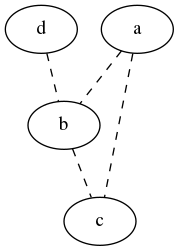
\includegraphics[scale=0.6]{dot/dot_extend_1.png}
     
      \caption{Startgraph}
      \label{fig:algo:extend:1}
   \end{subfigure}&
   \begin{subfigure}[b]{0.32\textwidth}
      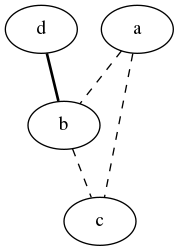
\includegraphics[scale=0.6]{dot/dot_extend_2.png}
     
      \caption{Kante (d,b) wird erfolgreich hinzugefügt}
      \label{fig:algo:extend:2}
    \end{subfigure}&
    \begin{subfigure}[b]{0.32\textwidth}
       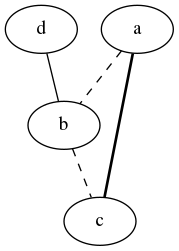
\includegraphics[scale=0.6]{dot/dot_extend_3.png}
    
      \caption{Kante (a,c) erfolgreich wird hinzugefügt}
      \label{fig:algo:extend:3}
    \end{subfigure}
  \end{tabular}
  
    \begin{tabular}[c]{ccc}
    \begin{subfigure}[b]{0.32\textwidth}
     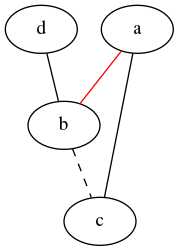
\includegraphics[scale=0.6]{dot/dot_extend_4.png}
    
      \caption{Kante (a,b) kann nicht hinzugefügt werden}
      \label{fig:algo:extend:4}
   \end{subfigure}&
   \begin{subfigure}[b]{0.32\textwidth}
    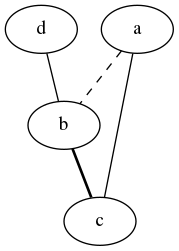
\includegraphics[scale=0.6]{dot/dot_extend_5.png}
      \caption{Kante (b,c) kann nicht hinzugefügt werden}
      \label{fig:algo:extend:5}
    \end{subfigure}&
    \begin{subfigure}[b]{0.32\textwidth}
     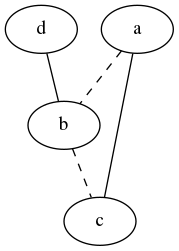
\includegraphics[scale=0.6]{dot/dot_extend_6.png}
    
      \caption{Resultierender Graph}
      \label{fig:algo:extend:6}
    \end{subfigure}
  \end{tabular}
  \caption{Beispielweiser Ablauf des Extends}\label{fig:algo:extend}
\end{figure}

\subsection{GRASP}
Nach dem experimentellen Untersuchen der Forward und Backward-Ansätze wurden deren Stärken und Schwächen deutlich. So kam auch die Idee diese beiden Ansätze zu kombinieren. Nach dem Planen und der Umsetzung einer solchen kombinierten Heuristik, hat die Recherche ergeben, dass es eine sehr ähnliche Art von Algorithmen bereits beschrieben wurde und unter dem dem Namen GRASP (Greedy Randomized Adaptive Search Procedure) \cite{Feo95} \cite{Bastos2014} bekannt ist. Es ist eine iterative Vorgehensweise wobei jede Iteration aus zwei Phasen besteht: 
\begin{itemize}
\item \textbf{Konstruktions-Phase.} Es wird mit einem leeren Graphen angefangen und nach und nach werden Knoten/Kanten nach einem bestimmten Kriterium hinzugefügt.
\item \textbf{Lokale Suche.} Da die Lösung, die in der Konstruktions-Phase generiert wurde, meistens nicht optimal ist, auch nicht in der einfachen Nachbarschaft. Deswegen wird in der lokalen Suche versucht die Lösung zu verbessern, indem man nach und nach die derzeitige Lösung durch eine bessere Lösung in der Nachbarschaft ersetzt.
\end{itemize}
Dieser GRASP Ansatz wurde auch schon erfolgreich für das Biclustering-Problem verwendet \cite{De12}.

Unsere Ansätze unterscheidet sich darin von den GRASP-Algorithmen, dass wir nicht in jeder Iteration einen neuen Graphen konstruieren, sondern auf dem bereits konstruierten Graphen weiter arbeiten. 

\subsubsection{Grow-Reduce}
Der Grow-Reduce-Ansatz sieht wie folgt aus: Begonnen wird mit einem Graphen, der die selben Knoten wie der Eingabegraph hat, aber keine Kanten. Dann wird in jeder Iteration ein Knoten und seine Umgebung hinzugefügt und durch lokale Suche werden alle neu entstandenen verbotenen Subgraphen wieder entfernt. Dies ist im Algorithmus \ref{algo:growReduce} zu sehen. 

Die Grow-Phase ist mit der Konstruktion-Phase des GRASP-Ansatzes vergleichbar und die Reduce-Phase mit der lokalen Suche.

\begin{algorithm}
  \captionof{algorithm}{GrowReduce}\label{algo:growReduce}
\begin{algorithmic}[1]
\Function{GrowReduceSolve}{\vars{G}, \vars{forbidden}}
	\State{\vars{graph} $\gets$ $(V(\vars{input}),\emptyset)$}
	\State{\vars{nodes} $\gets$ \func{order}(V(\vars{G}))}
	\For{\vars{node} $\in$ \vars{nodes}}
		
		\For{\vars{neighbor} $\in$ N(\vars{node})}\Comment{Grow Phase}
			\State{Add Edge (\vars{node}, \vars{neighbor}) to \vars{graph}}
		\EndFor
		\For{\vars{f} $\in$ \vars{forbidden}}\Comment{Reduce Phase}
			\State{\vars{forbiddenSubgraph} $\gets$ \func{findFS}(\vars{graph},\vars{f})}
			\While{\vars{forbiddenSubgraph} != $\emptyset$}
				\State{\vars{edge} $\gets$ random Edge from \vars{forbiddenSubgraph}}
				\State{\vars{count} $\gets$ \#(\func{findAllFS}(\vars{graph},\vars{f}))}
				\State{flip \vars{edge} in \vars{graph}}
				\State{countAfter $\gets$ \#(\func{findAllFS}(\vars{graph},\vars{f}))}
				\If{\vars{countAfter} $\geq$ \vars{count}}
					\State{flip \vars{edge} in \vars{graph}}
				\EndIf
				\State{\vars{forbiddenSubgraph} $\gets$ \func{findFS}(\vars{graph}, \vars{f})}
			\EndWhile
		\EndFor
		
	\EndFor
\Return{\vars{graph}}
\EndFunction
\end{algorithmic}
\end{algorithm}

\subsubsection{Explored-Grow-Reduce}
Der Explored-Grow-Reduce-Ansatz ist dem Grow-Reduce-Ansatz ähnlich, bis auf das, es in der Grow-Phase nur die Kanten zu Knoten hinzufügt, die bereits erforscht sind.

Dieser Unterschied wird in der Abbildung \ref{fig:algo_explored} verdeutlich, wo nur die Grow Schritte visualiert wurden, ohne die Reduce-Phase, um es zu vereinfachen.In Abbildung \ref{fig:algo_explored_1} ist der Anfangstatus zu sehen. Die gestrichelten Kanten, sind Kanten die Graphen vorhanden sind, aber noch nicht hinzugefügt worden sind und es wird der Knoten $a$ hinzugefügt, weil aber keine anderen Knoten bisher hinzugefügt worden sind, wird  werden keine Kanten hinzugefügt.
In Abbildung \ref{fig:algo_explored_2} wird der Knoten $b$ hinzugefügt und weil $a$ auch schon hinzugefügt wurde, wird auch die Kante $(a,b)$ hinzugefügt. Aber weder $(a,c)$ noch $(a,b)$ werden hingefügt, weil $c$ noch nicht erforscht wurde.
In Abbildung \ref{fig:algo_explored_3} wird der Knoten $c$ hinzugefügt und somit auch die Kanten $(a,b)$ und $(a,c)$.
	
	
\begin{figure}
  \centering
  \begin{tabular}[c]{ccc}
    \begin{subfigure}[b]{0.32\textwidth}
      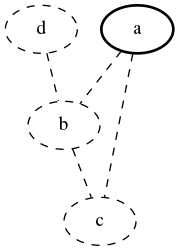
\includegraphics[scale=0.5]{dot/dot_explored_1.png}
     
      \caption{Knoten a wird hinzugefügt}
      \label{fig:algo_explored_1}
   \end{subfigure}&
	 \begin{subfigure}[b]{0.32\textwidth}
	   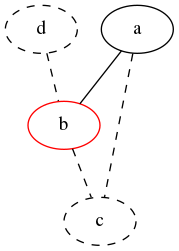
\includegraphics[scale=0.5]{dot/dot_explored_2.png}
	    \caption{Knoten b wird hinzugefügt}
	    \label{fig:algo_explored_2}
	  \end{subfigure}&
    \begin{subfigure}[b]{0.32\textwidth}
      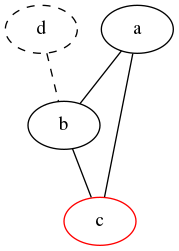
\includegraphics[scale=0.5]{dot/dot_explored_3.png}
	 
	    \caption{Knoten c wird hinzugefügt}
	    \label{fig:algo_explored_3}
    \end{subfigure}
  \end{tabular}
  \caption{Beispielweise Grow-Phase}\label{fig:algo_explored}
\end{figure}

\begin{algorithm}
  \captionof{algorithm}{ExploredGrowReduce}\label{algo:ExploredGrowReduce}
\begin{algorithmic}[1]
\Function{ExploredGrowReduceSolve}{\vars{input}, \vars{forbidden}}
	\State{\vars{graph} $\gets$ $(V(\vars{input}),\emptyset)$}
	\State{\vars{nodes} $\gets$ \func{order}(V(\vars{input}))}
	\State{\vars{explored} $\gets \emptyset$}
	\For{\vars{node} $\in$ \vars{nodes}}
		
		\For{\vars{neighbor} $\in$ N(\vars{node})}\Comment{Grow Phase}
			\If{\vars{neighbor} $\in$ \vars{explored}}
				\State{Add Edge (\vars{node}, \vars{neighbor}) to \vars{graph}}
			\EndIf
		\EndFor
		\State{\vars{explored} $\gets$ \vars{explored} $\cup$ $\{$\vars{node}$\}$}
		\For{\vars{f} $\in$ \vars{forbidden}}\Comment{Reduce Phase}
			\State{\vars{forbiddenSubgraph} $\gets$ \func{findFS}(\vars{graph},\vars{f})}
			\While{\vars{forbiddenSubgraph} != $\emptyset$}
				\State{\vars{edge} $\gets$ random Edge from \vars{forbiddenSubgraph}}
				\State{\vars{count} $\gets$ \#(\func{findAllFS}(\vars{graph},\vars{f}))}
				\State{flip \vars{edge} in \vars{graph}}
				\State{countAfter $\gets$ \#(\func{findAllFS}(\vars{graph},\vars{f}))}
				\If{\vars{countAfter} $\geq$ \vars{count}}
					\State{flip \vars{edge} in \vars{graph}}
				\EndIf
				\State{\vars{forbiddenSubgraph} $\gets$ \func{findFS}(\vars{graph}, \vars{f})}
			\EndWhile
		\EndFor
		
	\EndFor
\Return{\vars{graph}}
\EndFunction
\end{algorithmic}
\end{algorithm}
\subsubsection{Sortierung der Knoten}
Sowohl in dem Grow-Reduce als auch dem Explorer-Grow-Reduce Algorithmus werden die Knoten mittels der Funktion \func{order} sortiert  und dann eine nach der anderen abgearbeitet. Nun kann man die Knoten nach unterschiedlichen Kriterien sortieren.
Es wurden 3 Sorterierungsfunktionen verwendet:
\begin{itemize}
\item Zufällig. Das ist einfachste und offensichtliches Sortierungsfunktion. Wenn keine Informationen über die Struktur der Daten vorhanden sind, dann ist das zufällige Abarbeiten der Knoten naheliegend.
\item Anzahl der Nachbarn. Die Knoten werden nach der Anzahl der Nachbarn im Eingabegraphen sortiert.
\item Anzahl von verbotenen Teilgraphen. Die Knoten werden danach sortiert, wie oft der Knoten in einem verbotenen Teilgraphen vorkam.
\end{itemize}
Bei den letzten beiden Sortierunsgmöglichenkeiten gibt es sowohl die aufsteigende und absteigende Variante. 

\subsection{Lineare Programmierung}
\subsubsection{Lineare Optimierung}
Bei der linearen Optimierung wird eine lineare Zielfunktion minimiert bzw. maximiert, wobei sie durch lineare Gleichungen und Ungleichungen beschränkt ist.
\subsubsection{Das Model des Graphen}
Wir nutzen binäre Variablen $e_{uv}$, wobei $u,v \in V$ sind und $u < v$ gilt.
Dabei ist $e_{uv} = 1$ genau dann wenn, die kante ${u,v}$ ein Teil des Lösungsgraphen ist.

Wir minimieren \[\sum_{u,v \in V} 
\begin{cases} 
      e_{u,v} & \{u,v\} \in E \\
      -e_{u,v} & \{u,v\} \notin E
   \end{cases}\]
Dies ist die Zielfunktion \vars{objective} im Algorithmus \ref{algo:blp}.

Da alle möglichen Bedingungen hinzuzufügen, welche bei alle verbotenen Subgraphen ausschließen würden, viel zum umfangreich wäre, werden die Bedingungen iterative dort hinzugefügt, wo es einen verbotenen Teilgraphen gibt (siehe Zeile \ref{algo:blp:add}). Dann wird der Problem gelöst(siehe Zeile \ref{algo:blp:solve}) und und die Änderungen auf den Graphen übertragen(siehe Zeile \ref{algo:blp:apply}) . Dann wird wieder nach alle verboteten Subgraphen gesucht(siehe Zeile \ref{algo:blp:findFS}). Dies wird solange wiederholt bis es keine mehr gibt. Nun ist die minimale Anzahl von Änderungen gefunden. 
Dieses Vorgehen ist im Algorithmus \ref{algo:blp} zu sehen.
\begin{algorithm}
  \captionof{algorithm}{F-Free BLP}\label{algo:blp}
\begin{algorithmic}[1]
\Function{solveBLP}{\vars{graph}, \vars{forbidden}}
\State{\vars{constraints} $\gets$ $\emptyset$}
\For{graph \vars{f} $\in$ \vars{forbidden}}
	\While{\func{findFS}(graph, f) != $\emptyset$}\label{algo:blp:findFS}
	  
		\For{each graph M $\in$ \func{findeFS}(\vars{graph}, \vars{f}) } \label{algo:blp:add}
			\State{contstraint $\gets$ 0}
			\For{each $\{u,v\}$ $\in$ E(M)} \Comment{Add all Constraints}
				\If{$\{u,v\}$ $\in$ E(graph)} 
					\State{contstraint += 1 - $e_{uv}$} 
				\Else 
					\State{contstraint += $e_{uv}$} 
				\EndIf
			\EndFor
			\State{\vars{constraints} $\gets$ \vars{constraints} $\cup$ \{ \vars{constraint} \}}
		\EndFor
		\State{\vars{variables} $\gets$ \func{lpSolve}(\vars{constraints}, \vars{objective})}\label{algo:blp:solve}
		\For{$e_{u,v}$ $\in$ \vars{variables}} \Comment{Apply solution to the graph.}\label{algo:blp:apply}
		  \If{$e_{u,v} = 1$}
		    \State{Set edge $(u,v)$ in \vars{graph}}
		  \Else
		    \State{Remove edge $(u,v)$ in \vars{graph}}
		  \EndIf
		\EndFor
	\EndWhile
\EndFor
\Return{graph}
\EndFunction
\end{algorithmic}
\end{algorithm}



\section{Aufbau der Test}

\label{sec:tests}
\subsection{Datensätze}
Folgende Datensätze wurden verwendet. Da verschiedene Mengen von verbotenen Teilgraphen monotonen Grapheneigenschaften zugeordnet werden können und jeder Datensatz von Graphen und jede Methode zufällige Graphen zu erzeugen, charakteristische Eigenschaften hat, ist es notwendig verschiedene Datensätze zu verwenden und verschiedenen Methoden zur Erzeugung von zufälligen Graphen.
Ingesammt wurde 5 verschiedene Methoden zur Erzeugung von zufälligen Graphen verwendet und 3 Datensätze.
Wir brachten zuerst die zufälligen Graphen.


\subsubsection{Barabási–Albert}
Für den Datensatz \vars{barabasi albert} wurde das Barabási–Albert Modell verwendet, welches ein zufälliges skalenfreies Netz erzeugt\cite{Albert02}.
Skalenfrei bedeutet hier, dass die Knotengrad einer Potenzverteilung folgt. Es gibt also viel mehr Konten die einen geringeren Grad haben als Knoten mit einem hohen Anzahl von Nachbarn. 

Es wurden 56 Graphen generiert mit Knotenanzahl in $\{10,20,30…140\}$, mit dem Parameter $m \in \{1,3,5,7\}$, welcher die Anzahl der der Kanten definiert, die zu bereits bestehenden Knoten erstellt werden.
\subsubsection{Erdős-Rényi}
Für den Datensatz \vars{ER} wurde das Erdős-Rényi Modell verwendet\cite{Gilbert59} \cite{Batagelj05}, wo jede Kante eine fixe Wahrscheinlichkeit hat zu existieren oder nicht zu existieren.

Es wurden dabei 54 Graphen generiert, mit einer Knotenanzahl $n \in \{10,20…,90\}$ und den folgenden Wahrscheinlichkeiten: $\frac{1}{10}$, $\frac{2}{10}$, $\frac{5}{20}$, $\frac{4}{10}$, $\frac{5}{10}$, $\frac{8}{10}$.


\subsubsection{Duplication-Divergence}
Für den Datensatz \vars{duplication divergence} wurde das Duplication Divergence Modell verwendet\cite{Ispolatov05}, welches Interaktionsnetzwerke zwischen Proteinen modelliert. Ein Beispiel ist in Abbildung \ref{fig:duplication-divergence} zu sehen.

Dabei gibt es in jeder Iteration bei der Erstellung eines solchen zufälligen Graphen zwei Phasen. Die erste ist die Duplikations-Phase, wo ein zufälliger Knoten $u$ genommen und dupliziert wird zu $v$. Dann beginnt die Divergence-Phase, wo zu jedem Nachbarn von $u$ mit gewissen Wahrscheinlichkeit $p$ eine Kante zu $v$ hinzugefügt wird. Falls keine Kanten hinzugefügt wurde, dann wird $v$ wieder gelöscht. Dies wird $n$-mal wiederholt 

Es wurden mit diesem Modell 54 Graphen generiert mit $n \in \{10,20…,90\}$ . Für die Wahrscheinlichkeiten $p$ wurden folgenden Werte verwendet $\frac{1}{10}$, $\frac{2}{10}$, $\frac{5}{20}$, $\frac{4}{10}$, $\frac{5}{10}$, $\frac{8}{10}$.
\begin{figure}
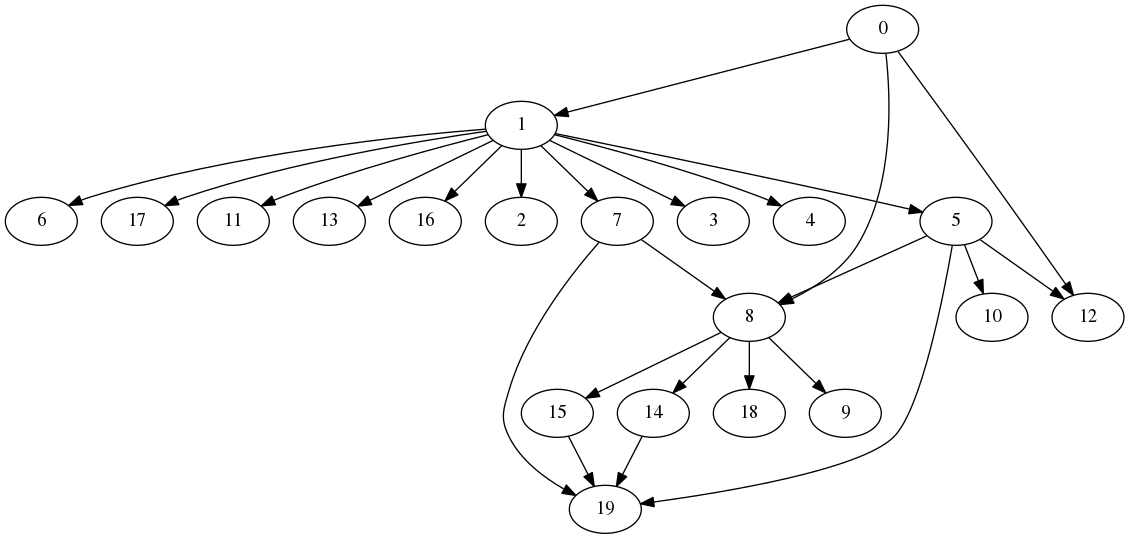
\includegraphics[scale=0.35]{dot/dot_dupdivergence.png}
\caption{Ein beispielhafter Duplication-Divergence Graph mit $n$ = 20 und $p$ = 0,4}
\label{fig:duplication-divergence}
\end{figure}

\subsubsection{Newman-Watts-Strogatz}
Für den Datensatz \vars{newman\_watts\_strogatz} wurde das Newman-Watts-Strogatz Modell verwendet\cite{Newman99}, welches Kleine-Welt-Graphen erzeugt mit geringen durchschnittlichen Knotendistanzen und einem hohen Clusterkoeffizienten.

Dabei wird zuerst ein Ring von $n$ Knoten erstellt. Dann wird jeder Knoten mit $k$ von seinen nächsten Nachbarn verbunden (oder mit $k-1$, wenn $k$ ungerade ist).
Dann werden Abkürzungen erzeugt indem, man für jede Kante $(u,v)$ in dem zugrundeliegenden $n$-Ring mit den $k$ nächsten Nachbarn: Füge mit der der Wahrscheinlichkeit $p$ eine neue Kante $(u,w)$ ein, wobei $w$ ein zufällig gewählter Knoten ist.

Es wurden mit diesem Model 144 Graphen generiert mit einer Knotenanzahl $n \in \{10,20…,90\}$  , $m \in \{2,4,6,8\}$ und der Wahrscheinlichkeit $p \in \{\frac{2}{10},\frac{4}{10},\frac{6}{10},\frac{8}{10}\}$.
\subsubsection{Powerlaw-Baum}
Für den Datensatz \vars{powerlaw}, wurde ein Modell verwendet, dass einen Baum erzeugt, dessen Knotengrad einer Potenzverteilung folgt. Ein Beispiel ist in Abbildung \ref{fig:powerlaw-tree} zu sehen.
Es wurden mit diesem Model 30 Graphen generiert mit einer Knotenanzahl zwischen $n \in \{10,15,20…,155\}$.
\begin{figure}
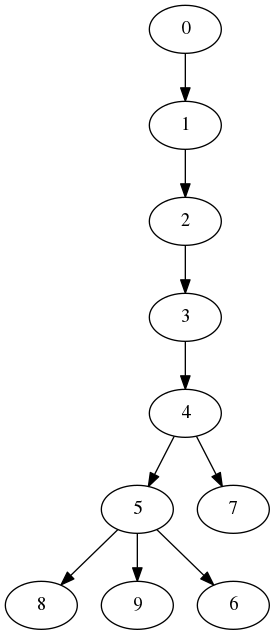
\includegraphics[scale=0.35]{dot/dot_powerlaw.png}
\caption{Ein Powerlaw-Baum mit $n$ = 10}
\label{fig:powerlaw-tree}
\end{figure}

\subsubsection{Netzwerke}
Für den Datensatz \vars{UCINetworkDataRepository} wurden 9 reale Graphen verwendet, bereitgestellt von der University of California.
\begin{itemize}
\item Der Graph \vars{karate} ist ein soziales Netzwerk von Freundschaften zwischen 34 Mitgliedern eines Karate-Clubs in einer US-Universität in 1970 \cite{Zachary77}.
\item Der Graph \vars{polbooks.paj} ist ein Netzwerk von Bücher über die aktuelle US Politik, die von dem Onlinehänder Amazon.com verkauft wurdem. Kanten repräsentieren häufiges Kaufen von den beiden Büchern von dem selben Käufer \cite{polbooks}.+

\item Der Graph \vars{football} ist ein Netzwerk von amerikanischen Footballspielen im Herbst 2000 \cite{Girvan02}.

\item Der Graph \vars{power.paj} ist ein Netzwerk, dass die Topologie des "Western States Power Grid" in der Vereinigten Staaten wiederspieglt  \cite{Watts98}.

\item Der Graph \vars{adjnoun} ist ein Netzwerk von häufigen Adjektiven und Nomen in dem Roman "David Copperfield" von Charles Dickens \cite{Newman06}.

\item Der Graph \vars{lesmiserables} ist ein Netwerke von Figuren, die in dem  Roman "Les Misérables" von Victor Hugo, zur gleichen Zeit auftreten \cite{Knuth93}. 


\item Der Graph \vars{celegansneural.paj} welches das neurale Netzwerk von Caenorhabditis elegans \cite{Watts98}. Es ist ein Fadenwurm, welcher gerne als Modellorganismus studiert wird. Jeder erwachsene C. elegans hat genau 302 Nervenzellen.


\item Der Graph \vars{dolphins} ist ein soziales Netzwerk von 62 Dolphinen die in einer Gemeinschaft in der Nähe von Neuseeland leben \cite{Lusseau03}. 

\item Der Graph \vars{polblogs} ist ein Netzwerk von Hyperlinks zwischen Webblogs in 2005, die sich mit auf US Politik beschäftigten \cite{Adamic05}.
\end{itemize}






\subsubsection{Squenzähnlichkeit von Proteinen}
Der Datensatz  \vars{bio1} umfasst 147 Graphen und der \vars{bio2} umfasst 350 Graphen. Beide sind Grahen die Squenzähnlichkeit von Proteinen modellieren \cite{Rahmann07} \cite{Bocker08}.

\subsection{Optimale Lösung}
Um die Qualität der Lösung eines heuristischen Ansatzes bewerten zu können, ist es sehr gut die optimale Lösung zu wissen. Es gibt verschiedene Ansatz wie das Problem zu lösen sein, wir haben uns jedoch für die lineare Optimierung entschieden. Der BLP-Alogoritmus versucht eine optimale Lösung zu finden. Dies kann jedoch sehr lange dauern, da die Komplexität des Problemes exponentiell. 
In der Tabelle Tabelle \ref{tab:size_solved_bio2} sehen wir, dass für viele verbotene Teilgraphen wir für alle Instanzen eine optimale Lösung berechnen konnten, aber es gibt schwierige verbotene Teilgraphen wie ($P_5$, triangle) wo man wir für die meisten Instanzen keine optimale Lösung haben.
\begin{center}
\captionof{table}{Nicht gelöste Instanzen für den Datensatz $bio2$}
\label{tab:size_solved_bio2}
\begin{tabular}{ccc}
\hline 
Verbotener Teilgraph & Anzahl & Prozent \\ 
\hline
$2 P_3$ & 0 & 0\% \\ 
$C_4$ & 0 & 0\% \\ 
claw & 0 & 0\% \\ 
paw & 4 & 1\% \\ 
triangle & 11 & 3\% \\ 
splitcluster & 26 & 7\% \\ 
($P_4,C_4)$ & 37 & 10\% \\ 
(x172, triangle) & 129 & 36\% \\ 
($P_5$, triangle)& 309 & 86\% \\ 
\hline
\end{tabular} 
\end{center}


\section{Implementation}

\label{sec:implementation}
\subsection{Repräsentation vom Graphen}
Die Graphen werden in einer Adjazenzmatrix gespeichert.

TODO: MORE

\subsection{Das Finden von induzierten Subgraphen}
Das Finden von induzierten Subgraphen ist der Teil der Algorithmen, der am zeitaufwändigsten ist und auf häufigsten aufgerufen wird. Deswegen ist hier die Wahl von dem richtigen Ansatz sehr wichtig. 

\subsubsection{Vergleich von Algorithmen fürs Finden von Ismorphen Subgraphen}
In diesem Abschnitt wollen wir drei Ansätze bezüglich ihrer Geschwindigkeit vergleichen. Um das ganze zu vereinfachen, testen wir Anwendungsfälle eines Ansatzes mit dem verbotenen Teilgraphen $P_3$. 

\begin{itemize}
\item Der erste ist VFLib. Es ist ein Bibliothekt, die mehrere Algorithmen jeweils für das Graphen Isomorphismus Problem, Graphen-Subgraph Isomorphismus Problem und das Graphen Monomorphimus Problem implementiert und zählt zu den schnellsten Implementationen \cite{Cordella04}.

\item Der zweite Ansatz nutzt die Boost-Implementation von VF2, welches VFLib auch implementiert.

\item Im dritten Ansatz wird die Suche nach dem $P_3$ selbst möglichst effizient implementiert. 
\end{itemize}

Hierbei vergleichen wir nicht die verschiedenen Algorithmen für das Graph-Subgraph Isomorphismus Problem, weil VFLib und Boost den selben grundlegenden Ansatz verwenden und die eigene Implentieren gar kein Graph-Subgraph Isomorphismus Algorithmus ist. Vielmehr geht es darum, herausfinden wie groß ungefähr der Overhead ist und wo es sich lohnt zu optimieren.

Die drei Anwendungsfälle wären:
\begin{itemize}
 \item \textbf{Alle Finden}: Finde und gebe alle verbotenen Teilgraphen zurück
 \item \textbf{Alle Zählen}: Zählen wie viele verbotene Teilgraphen der Graph hat
 \item \textbf{Einen zurückgeben}: Finde einen verbotenen Teilgraphen und gebe ihn zurück.
\end{itemize}

In der Tabelle \ref{tab:benchmark_isomorph} werden die Resultate anzeigt, dabei gibt die Zeit an wie lange es gebraucht hat die Aufgabe auf allen 147 Graphen von dem Datensatz \vars{bio1} auszuführen. In der Zeit ist die Zeit für das Einlesen der Graphen nicht mit einbegriffen. Die Werte unter der Zeit, sind Angaben, wie viel mal langsamer der Ansatz als der schnellste Ansatz ist.
\begin{table}

\centering

\begin{tabular}{c ccc}
\hline 
Verfahren & Alle finden & Alle zählen & Einen zurückgeben \\ 
\hline 
VFLib & 1,73s (2,4x) & 0,87s (22x) & 0,0124s (77x) \\ 
Boost & 3,04s (4,2x) & 1,68s (42x) & 0,00102s (6,4x) \\ 
Naive P3-Suche & 0,73s & 0,04s & 0,00016s \\ 
\hline 
\end{tabular} 
\caption{Benchamrk}
\label{tab:benchmark_isomorph}
\end{table}
Zu sehen ist, dass die "Naive P3-Suche" viel schneller ist, aber es ist zu bebachten, dass VFLib und Boost allgemeine Ansätze sind, während unse nur für den Graphen $P_3$ funktioniert. 

Zu beobachten ist auch, dass VFLib bei dem \glqq Alle finden\grqq \, und \glqq Alle zählen\grqq \, deutlich schneller ist, aber beim \glqq Einen zurückgeben\grqq \, weitaus langsamer ist. Dies hat mit dem Benchmark selbst zu tun. Weil dort die Algorithmen sehr schnell sind, wurde es 100-mal auf jedem Graphen ausgeführt. Dann wurde die Zeit durch 100 dividiert. 
An sich ist es auch kein Problem, aber der Unterschied liegt in der Tatsache, dass die Datenstruktur von von VFLib unveränderlich ist und wir bei jedem Aufruf einen neuen Graphen für VFLib erstellen, während bei Boost wir den Graphen nicht immer wieder neu erstellen müssen. Auch wenn man den Benchmark anders gestalten könnte, wurde er absichtlich so gestaltet, weil es in den Heuristiken eine reale Anwendung ist: Oft wird wiederholt eine Änderung gemacht und dann nach einem verbotenen Teilgraphen gesucht. Hier wäre der Boost-Ansatz also weitaus besser, weil man nach einer jeder Änderung nicht einen neuen Graphen konstruieren müsste.

Die Schlussfolgerung von diesem Benchmark ist, dass die VFLib und Boost Algorithmen schnell genug sind und höchstens eine Optimierung von \glqq   Alle zählen\grqq \, eine Option wäre, die auch vielversprechend wäre.

\section{Auswertung}
\label{sec:results}

Zuerst eine grober Vergleich.


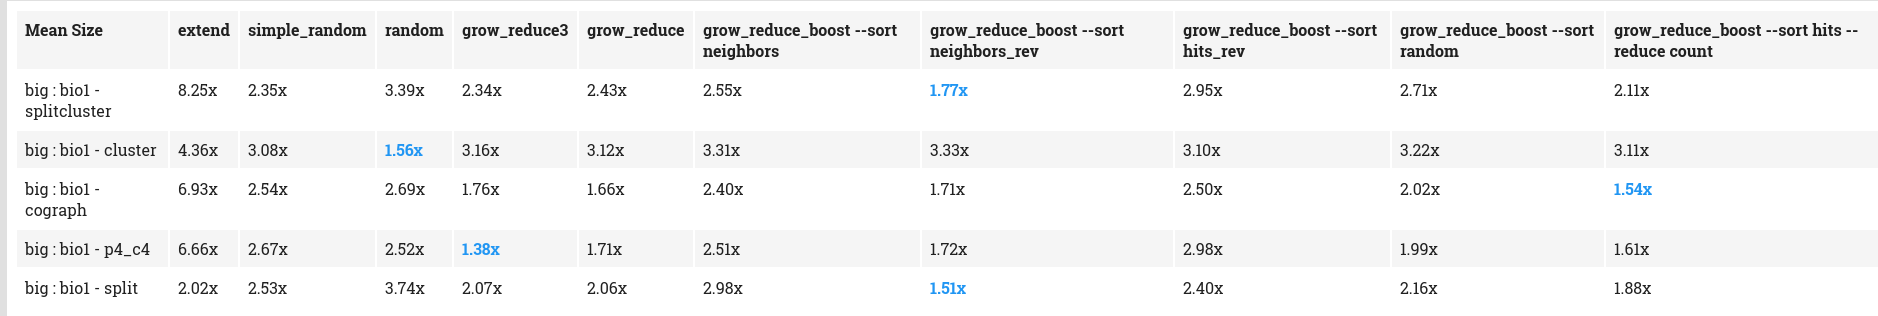
\includegraphics[scale=0.3]{plots/table_all.png}

\subsection{Backward-Ansatz}
\subsection{Forward-Ansatz}
\subsection{Grow-Reduce-Ansatz}


\subsection{Vergleich mit anderen Heuristiken}
\label{sec:compare}

\subsubsection{Cluster-Editing}
Die 2K-Heuristik basiert auf einem Kernel für das Cluster-Editing-Problem, welches maximal 2K Knoten liefert \cite{Chen12}. Wenn man dort eine Bedingung für die Reduktionsregel  abschwächt, kommt eine gute Heuristik für das Cluster-Editing-Problem heraus. Dabei wird die Bedingung mit jedem Durchlauf abgeschwächt.
\pagebreak
\begin{center}
  \captionof{algorithm}{2K Heuristik}\label{algo:2k}
\begin{algorithmic}[1]
\Function{solve2K}{\vars{g} :: Gewichteter Graph}
\State{\vars{x} $\gets$ 1,0} 
\While{\vars{g} has a P3}
	\For{each knoten \vars{u} $\in$ \vars{g}}
		\If{$2 \cdot x \cdot costClique(g, u) + x \cdot costCut(g, u) < \#(N(u))$}
			\For{each $\{a,b\}$  mit $a \in N(u)$, $b \in N(u) \land a \neq b$}
				\State{\func{merge}(a,b)}
			\EndFor
		\EndIf
	\EndFor
	\State{$\vars{x} \gets$ $0,99 \cdot \vars{x} - 0,01$}
\EndWhile

\Return{graph}
\EndFunction

\Function{costClique}{graph :: Gewichteter Graph, u :: Kante}
\State{cost $\gets$ 0}
	\For{each $\{a,b\}$  mit $a \in N^{*}(u)$, $b \in N^{*}(u) \land \{a,b\} \notin graph$}
		\State{cost += $|\,w(\{a,b\})\,|$}
	\EndFor

\Return{cost}
\EndFunction
\Function{costCut}{graph :: Gewichteter Graph, u :: Kante}
\State{cost $\gets$ 0}
	\For{each $\{a,b\}$  mit $a \in N^{*}(u)$, $b \notin N^{*}(u) \land \{a,b\} \in graph$}
		\State{cost += $w(\{a,b\})$}
	\EndFor

\Return{cost}
\EndFunction
\end{algorithmic}
\end{center}


\begin{center}
\captionof{table}{Vergleich der durchschnittlichen Lösungsgröße}
\label{tab:size_2k}
\begin{tabular}{c|c c|c c} 
& \multicolumn{2}{c|}{Aprox2k} & \multicolumn{2}{c}{ExploredGrowReduce\footnote{Siehe Algorithmus \ref{algo:ExploredGrowReduce} mit 5 Iterationen }} \\ 
Datensatz & \multicolumn{1}{c}{mean}  &  \multicolumn{1}{c|}{std} &  \multicolumn{1}{c}{mean} &  \multicolumn{1}{c}{std} \\ 
\hline 
bio1 \footnote{Testergebnis: 2016-04-20 17:29:08} & \textbf{43.44}  & 79.81 & 133.59 & 249,62 \\ 
bio2 \footnote{Testergebnis: 2016-04-20 17:31:40} & \textbf{34.11} & 19.79 & 113.81 & 166,01 \\ 
duplication-divergence \footnote{Testergebnis: 2016-04-20 17:36:40} & 155.17 & 217.38 & \textbf{92.30} & 115,22 \\ 
newman-watts-strogatz \footnote{Testergebnis: 2016-04-20 17:36:57} & 165.22 & 149,86 & \textbf{152.34} & 127,51 \\ 
albert-barabasi \footnote{Testergebnis: 2016-04-20 17:38:17} & 324.30 & 316,32 & \textbf{248.84} & 226,87 \\ 
binomial \footnote{Testergebnis: 2016-04-20 18:17:08} & \textbf{493.17} & 545,19 & 554.61 & 670,91 \\ 

\end{tabular} 
\end{center}


\subsubsection{Quasi-Threshold-Editing}


In \cite{BrandesHSW15} wurde ein neuer schneller und auch für große Graphen geeigneter Algorithmus entwickelt für das Quasi-Threshold Editing Problem. Quasi-Threshold Graphen, auch bekannt als trivial perfekte Graphen lassen sich auch als $(P_4, C_4)$ - freie Graphen charakterisieren. 

In Tabelle \ref{tab:qual_mover} wird die Lösungsqualität von dem Quasi-Thresold-Mover und unserem Algorithmus ExploredGrowReduce verglichen. In der Tabelle \ref{tab:size_mover} wird die durschnittliche Größe der Lösungen verglichen. 
Der Quasi-Threschold-Mover ist unserem Ansatz weit überlegen. 


\begin{center}
\captionof{table}{Vergleich der durchschnittlichen Lösungsqualität}
\label{tab:qual_mover}
\begin{tabular}{c|c c|c c}
& \multicolumn{2}{c|}{ExploredGrowReduce\footnote{Siehe Algorithmus \ref{algo:ExploredGrowReduce} mit Standard-Parametern }} & \multicolumn{2}{c}{Quasi-Threshold-Mover} \\ 
Datensatz & \multicolumn{1}{c}{mean}  &  \multicolumn{1}{c|}{std} &  \multicolumn{1}{c}{mean} &  \multicolumn{1}{c}{std} \\ 
\hline 
bio1 \footnote{Testergebnis: 2016-04-20 12:46:35 } & 1.61x  & 1.30 & \textbf{1.05x} & 0.14 \\ 

bio2 \footnote{Testergebnis: 2016-04-20 12:53:45} & 1.69x & 1.03 & \textbf{1.05x} & 0.10 \\ 

duplication-divergence \footnote{Testergebnis: 2016-04-20 13:09:36} & 1.42x & 0.33 & \textbf{1.04x} & 0.05 \\ 

newman-watts-strogatz \footnote{Testergebnis: 2016-04-20 13:12:44} & 1.38x & 0.22 & \textbf{1.06x} & 0.05 \\ 

\end{tabular} 
\end{center}

\begin{center}
\captionof{table}{Vergleich der durchschnittlichen Lösungsgröße}
\label{tab:size_mover}


\begin{tabular}{c|c c|c c}


 & \multicolumn{2}{c|}{\textbf{ExploredGrowReduce}} & \multicolumn{2}{c}{\textbf{Quasi-Threshold-Mover}} \\ 
Datensatz & \multicolumn{1}{c}{mean}  &  \multicolumn{1}{c|}{std} &  \multicolumn{1}{c}{mean} &  \multicolumn{1}{c}{std} \\ 
\hline 
bio1 & 52.25  & 150.25 & \textbf{20.88} & 46.51 \\ 

bio2 & 23.12 & 19.91 & \textbf{13.89} & 9.64 \\ 

duplication-divergence & 73.87 & 117.35 & \textbf{51.46} & 80.23 \\ 

newman-watts-strogatz & 146.48 & 128.42 & \textbf{103.38} & 87.99 \\ 

\end{tabular} 
\end{center}

\section{Zusammenfassung}
\subsection{Anwendungen}
Auch ein möglicher Anwendungsfall wäre, dass man eine Menge von Graphen hat, die man noch nicht analysiert hat. Wenn man nun die Heuristiken mit vielen möglichen verbotenen Teilgraphen auf den Eingabegraphen laufen lässt und dann vergleicht, kann man sehen, welche Graphen welche Strukturen eher besitzen.

Um diesen Anwendungsfall zu demonstrieren. Wir testen jeweils 15 Graphen aus verschiedenen Quellen: Graphen die mit dem Duplication-Divergence Modell generiert wurden, Graphen die mit dem Powerlaw-Modell generiert wurden und und biologische Daten, die aus der Squenzähnlichkeit von Proteinen generiert wurden.
In der Abbildung \ref{fig:best-graph} ist die durschnittliche normalisierte Lösungsgröße der 3 Graphengruppen mit verschiedenen verbotenen Teilgraphen.

\begin{figure}
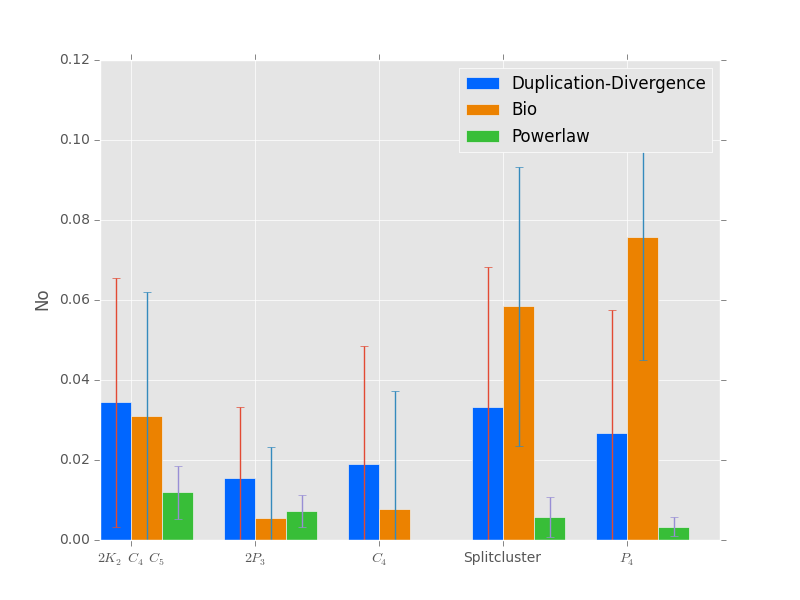
\includegraphics[scale=0.7]{plots/best.png} 
\caption{Durschnittliche normalisierte Lösungsgröße}
\label{fig:best-graph}
\end{figure}

So ist es zu erwarten, dass die Bearbeitungsdistanz zu $C_4$-freien Graphen 0 ist, weil es eben Bäume sind und dort es keine Zyklen gibt.
Auch ist die verhältnismäßige kleine Distanz zu $P_4$-freien Graphen in einem Powerlaw-Graphen nicht ungewöhnlich, denn es gibt wenige Knoten, die einen Knotengrad von 4 haben. Siehe auch Abbildung \ref{fig:powerlaw-tree} auf der Seite \pageref{fig:powerlaw-tree}.

Diese gerade getätigten Beobachtungen konnten wir tun, weil wir die Struktur der Powerlaw-Graphen kennen. Aber was können wir rausfinden, wenn wir uns die Duplication-Divergence-Graphen anschauen und sie mit den $bio$-Graphen vergleichen. 


\subsection{Zukünftige Forschungsmöglichkeiten}
\subsubsection{Besser Sortierung von Grow-Reduce}
\subsubsection{Besser Konvergenzkriterium}
\subsubsection{Obere Schranken}
\subsubsection{Untere Schranken}

\bibliographystyle{plain}
\bibliography{biblio}

\end{document}
